\begin{enumerate}
	\item Цель:
		\begin{itemize}
			\item Сделать резервуар, способный вместить в себе 5 больших шариков, оснастить его сервоприводом со стенкой, закрывающим резервуар и установить на робота.
			\item Придумать способ возвращения конструкции в изначальное положение.
			\item Написать программу для управления сервоприводом 
		\end{itemize}
	\item Реализация:
		\begin{itemize}
			\item Резервуар был сделан при помощи железной сетки и пластиковой вазы. При установке выяснилось, что контейнер слишком широкий и слишком сильно трется о внутреннюю поверхность подъемника. (Рисунки 21, 22)
			\item В качестве возвращающего механизма были использованы обычные канцелярские резинки(Рисунки19, 20)\\
			\begin{minipage}{0.3\linewidth}
			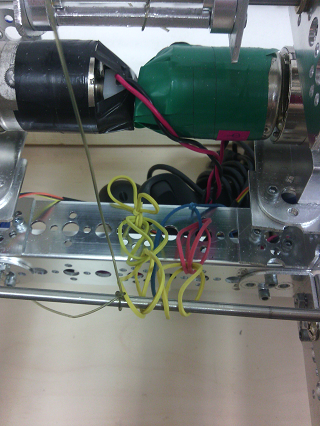
\includegraphics[width=45mm,height=45mm]{Days/15.11.14/12_1_robot}\\ Рисунок 19
			\end{minipage}
			\begin{minipage}{0.3\linewidth}
			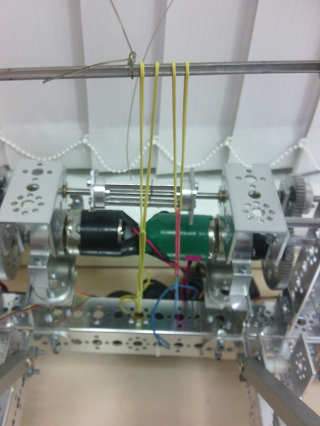
\includegraphics[width=45mm,height=45mm]{Days/15.11.14/12_2_robot}\\ Рисунок 20
			\end{minipage}\\
			\begin{minipage}{0.3\linewidth}
			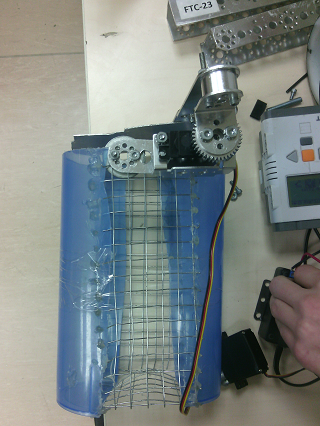
\includegraphics[width=45mm,height=45mm]{Days/15.11.14/12_3_robot}\\ Рисунок 21
			\end{minipage}
			\begin{minipage}{0.3\linewidth}
			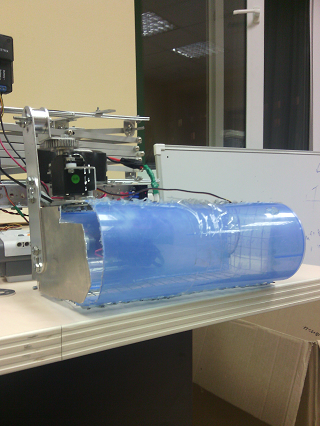
\includegraphics[width=45mm,height=45mm]{Days/15.11.14/12_4_robot}\\ Рисунок 22
			\end{minipage}\\
		\end{itemize}
	\item Идеи и планы:
		\begin{itemize}
			\item Закрепить резервуар на конструкции все же не удалось. На следующем занятии планируем сделать новый, меньшего размера и другой формы, закрепить его на конструкции и протестировать.
			\item Тренироваться.
		\end{itemize}
		\fillpage
\end{enumerate}